Gesucht ist für das Petrinetz



\begin{centering}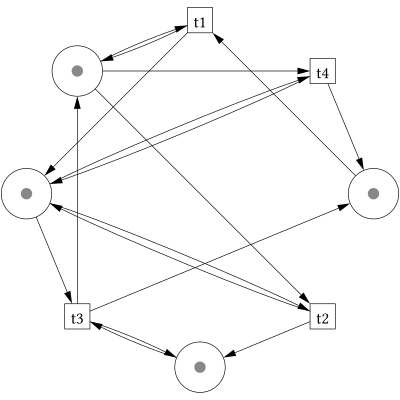
\includegraphics[min width=0.4\textwidth=0.6\textwidth,min height=0.4\textwidth=0.6\textwidth,keepaspectratio,max width=0.9\textwidth,max height=0.9\textwidth]{60/graph-1petri6798dd80b41d3221abe8bfcf7931ecef48ab6bc5eebe09d6a77c220768a60f7501013.pdf}\end{centering}

eine Transitionsfolge, durch welche die folgende Markierung erreicht wird:

\begin{centering}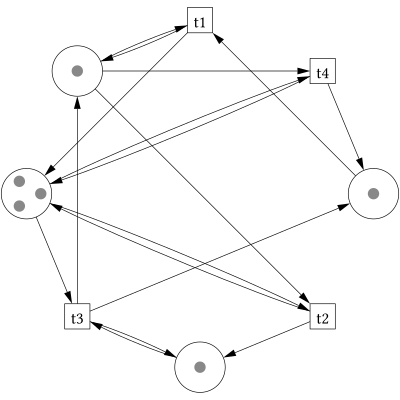
\includegraphics[min width=0.4\textwidth=0.6\textwidth,min height=0.4\textwidth=0.6\textwidth,keepaspectratio,max width=0.9\textwidth,max height=0.9\textwidth]{60/graph0petri18a6832a0ea325f8b83c352cdac8b029dd3b900696e925eeb0e69da1c00473ec01013.pdf}\end{centering}





Geben Sie Ihre Lösung als maximal 8-schrittige Auflistung der folgenden Art an:


\begin{minted}{text}
[t1, t2, t3]
\end{minted}
Wobei die Angabe dieser drei Schritte bedeuten soll, dass nach dem Schalten von t1, danach t2, und schließlich t3 (in genau dieser Reihenfolge), die gesuchte Markierung erreicht wird.

Hinweis: Es gibt keine Lösung mit weniger als 8 Schritten.

Bitte beachten Sie: Beim Bewegen über oder Klicken auf Kanten / Knoten bzw. ihre Beschriftungen werden die jeweils zusammengehörenden Komponenten hervorgehoben.